%
% nichthauptideal.tex
%
% (c) 2021 Prof Dr Andreas Müller, OST Ostschweizer Fachhochschule
%
\bgroup
\definecolor{darkgreen}{rgb}{0,0.6,0}
\begin{frame}[t]
\setlength{\abovedisplayskip}{5pt}
\setlength{\belowdisplayskip}{5pt}
\frametitle{Nicht-Hauptideal in $\mathbb{Z}[X]$}
\vspace{-20pt}
\begin{columns}[t,onlytextwidth]
\begin{column}{0.48\textwidth}
\begin{block}{Hauptideal\uncover<2->{ = ``Gerade''}}
\vspace{-10pt}
\begin{align*}
\langle X+1\rangle&=(X+1) = {\color{red}(X+1)\cdot\mathbb{Z}[X]}
\end{align*}
\begin{center}
\begin{tikzpicture}[>=latex,thick,scale=0.4]
\draw[->] (-6.3,0) -- (6.8,0) coordinate[label={$\mathbb{Z}$}];
\draw[->] (0,-6.2) -- (0,6.6) coordinate[label={right:$\mathbb{Z}X$}];
\foreach \x in {-6,...,6}{
	\fill[color=red] (\x,\x) circle[radius=0.12];
}
\end{tikzpicture}
\end{center}
\end{block}
\end{column}
\begin{column}{0.48\textwidth}
\uncover<3->{%
\begin{block}{Ideal mit zwei Erzeugenden}
\vspace{-10pt}
\begin{align*}
\uncover<6->{
{\color{darkgreen}
\langle 2,X\rangle
}
&=}
\uncover<5->{
{\color{red}2\cdot\mathbb{Z}[X]}
}
\uncover<6->{+}
\uncover<4->{
{\color{blue}X\cdot\mathbb{Z}[X]}
}
\end{align*}
\begin{center}
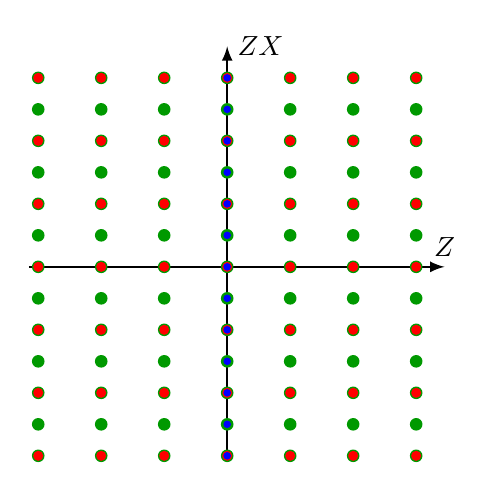
\begin{tikzpicture}[>=latex,thick,scale=0.4]
\draw[->] (-6.3,0) -- (6.9,0) coordinate[label={$\mathbb{Z}$}];
\draw[->] (0,-6.2) -- (0,7.0) coordinate[label={right:$\mathbb{Z}X$}];
\uncover<6->{
	\foreach \x in {-6,-4,...,6}{
		\foreach \y in {-6,...,6}{
			\fill[color=darkgreen] (\x,\y) circle[radius=0.20];
		}
	}
}
\uncover<5->{
	\foreach \x in {-6,-4,...,6}{
		\foreach \y in {-6,-4,...,6}{
			\fill[color=red] (\x,\y) circle[radius=0.16];
		}
	}
}
\uncover<4->{
	\foreach \y in {-6,...,6}{
		\fill[color=blue] (0,\y) circle[radius=0.12];
	}
}
\end{tikzpicture}
\end{center}
\end{block}}
\end{column}
\end{columns}
\end{frame}
\egroup
